\cleardoublepage{}

\chapter{相关技术}



\section{插入说明}

我们可以用 includegraphics 来插入现有的不同格式的图片,如图\ref{fig:ai-agent}。论文中尽量使用矢量图,如.pdf格式的图片

\begin{figure}[ht]
    \centering
    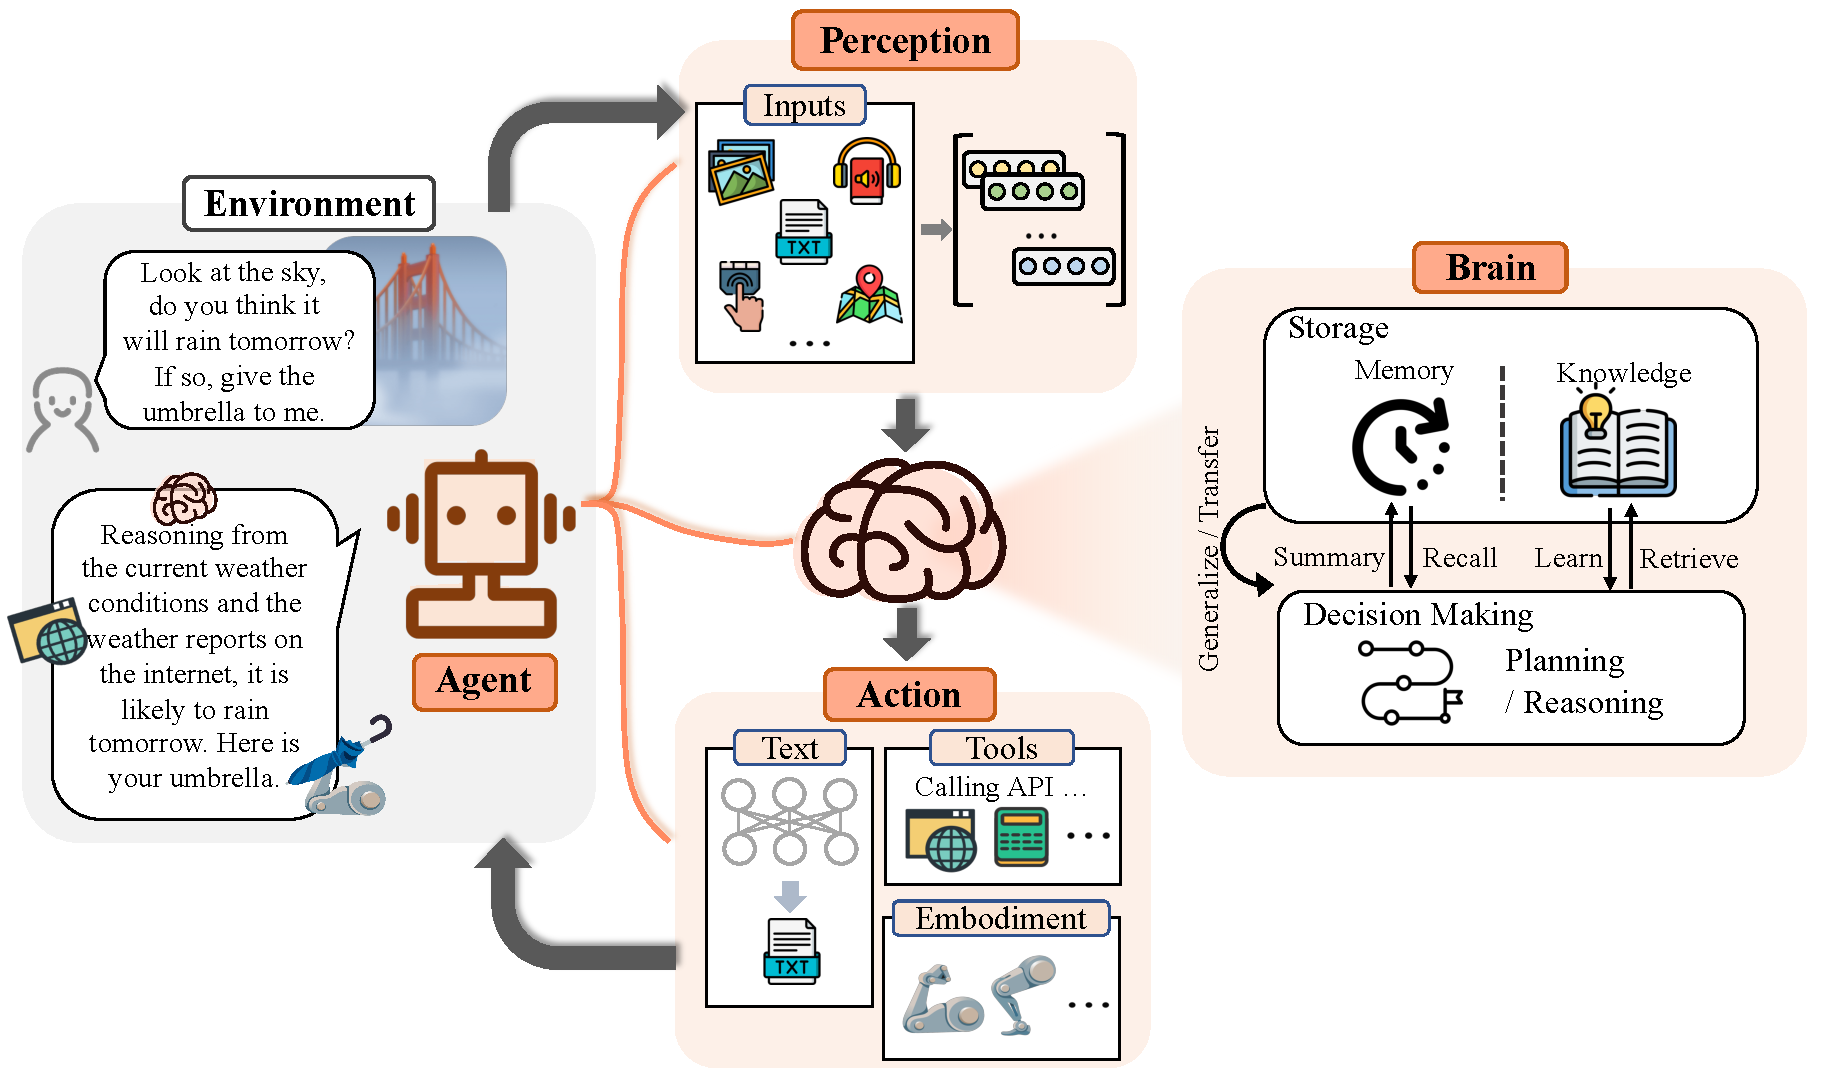
\includegraphics[width=.4\linewidth]{AI agent的组成.pdf}
    \caption{\label{fig:ai-agent}AI agent的组成.pdf}
\end{figure}

\par 如\ref{tab:compare}所示,这是一张自动调节列宽的表格。推荐两个常用的在线表格生成工具:Advanced Table Editor(\url{https://www.latex-tables.com/})和 Tables Generator(\url{https://www.tablesgenerator.com/})。


\begin{table}[ht]
	\footnotesize           
	\centering
	\caption{代码智能体相比 Text/JSON 在 LLM 动作上的优势}
	\label{tab:compare}
	\setlength\extrarowheight{2pt}  % 适度增大行距
	\begin{tabularx}{\textwidth}{lXX}
		\toprule
		& \textbf{代码智能体用于 LLM 动作} & \textbf{JSON 或 Text 用于 LLM 动作} \\
		\midrule
		预训练数据兼容性 & 有大量代码可用于预训练 & 需要针对特定格式进行数据整理 \\
		复杂操作支持 & 通过控制流和数据流原生支持 & 即便可行,也需要精心设计(例如定义新工具以模拟 if 语句) \\
		工具可用性 & 可以直接使用现有的软件包 & 需手动适配工具 \\
		自动反馈能力 & 反馈机制(如 traceback)作为基础机制已经在大多数编程语言中实现 & 需额外设计反馈流程 \\
		\bottomrule
	\end{tabularx}
\end{table}

\par 如\ref{equ:sample},这是一个公式

\begin{equation}
\label{equ:sample}
\mathrm{Logits}(t_n) = \mathrm{GenModel}\bigl(t_n \mid \{\mathrm{input}, t_1, \ldots, t_{n-1}\}\bigr)
\end{equation}

\par 如算法\ref{alg:sample},这是一个算法

\begin{algorithm}[ht]
	\caption{CodeAgent-based Workflow}
	\label{alg:sample}
	\begin{algorithmic}
		\State \textbf{memory} $\gets$ [user\_defined\_task]
		\While{llm\_should\_continue(memory)}
		\State $action \gets llm\_get\_next\_action(memory)$
		\State $observations \gets execute\_action(action)$
		\State $memory \gets memory + [action,\ observations]$
		\EndWhile
	\end{algorithmic}
\end{algorithm}

\par 这是一个无序列表

\begin{itemize}
    \item aaa
    \item bbb
    \item ccc
\end{itemize}

\par 这是一个有序列表(默认编号格式)

\begin{enumerate}
    \item aaa
    \item bbb
    \item ccc
\end{enumerate}

\par 下面是两个有序列表(自定义编号格式),你可以按照你的偏好设置

\begin{enumerate}[label=\arabic*)]	
    \item aaa
    \item bbb
    \item ccc
\end{enumerate}

\noindent\hrulefill

\begin{enumerate}[label=(\alph*)]
    \item athesiaa
    \item bbb
    \item ccc
\end{enumerate}

\subsection{文献引用}

文献引用可以使用两种方式,下面两种方式任选一个即可,但是需要全文统一

引用文献方式一:文献\cite{Chase_LangChain_2022}、文献\cite{wang2024executable}

引用文献方式二:文献\parencite{Elovic_gpt-researcher_2023}、文献\parencite{smolagents}

\subsection{关于代码}

\par 目前学院没有明确给出代码格式,你可以自己定义,也可以参照我的设置来使用
\begin{verbatim}
%复制以下代码到导言区
\definecolor{dkgreen}{rgb}{0,0.6,0}
\definecolor{gray}{rgb}{0.5,0.5,0.5}
\definecolor{mauve}{rgb}{0.58,0,0.82}

\lstset{ 
    language=python,                
    basicstyle=\footnotesize,       
    numbers=left,                   
    numberstyle=\tiny\color{gray}, 
    stepnumber=1,                   
    numbersep=5pt,                  
    backgroundcolor=\color{white}, 
    showspaces=false,              
    showstringspaces=false,         
    showtabs=false,                 
    frame=single,                   
    rulecolor=\color{black},        
    tabsize=2,                      
    captionpos=b,                   
    breaklines=true,                
    breakatwhitespace=false,        
    title=\lstname,                   
    keywordstyle=\color{blue},          
    commentstyle=\color{dkgreen},       
    stringstyle=\color{mauve},         
    escapeinside={\%*}{*)},            
    morekeywords={*,...}               
}
\end{verbatim}

\definecolor{dkgreen}{rgb}{0,0.6,0}
\definecolor{gray}{rgb}{0.5,0.5,0.5}
\definecolor{mauve}{rgb}{0.58,0,0.82}

\lstset{ 
    language=python,                
    basicstyle=\footnotesize,       
    numbers=left,                   
    numberstyle=\tiny\color{gray}, 
    stepnumber=1,                   
    numbersep=5pt,                  
    backgroundcolor=\color{white}, 
    showspaces=false,              
    showstringspaces=false,         
    showtabs=false,                 
    frame=single,                   
    rulecolor=\color{black},        
    tabsize=2,                      
    captionpos=b,                   
    breaklines=true,                
    breakatwhitespace=false,        
    title=\lstname,                   
    keywordstyle=\color{blue},          
    commentstyle=\color{dkgreen},       
    stringstyle=\color{mauve},         
    escapeinside={\%*}{*)},            
    morekeywords={*,...}               
}
上述设置最后生成的代码样式如下:

Java代码示例:
\begin{lstlisting}[language=java]
private void parseJSONWithJSONObject(String jsonData,SQLiteDatabase db){
    try {
        JSONObject jsonObject = new JSONObject(jsonData);
        JSONArray results;
        if(jsonObject.has("result")) results = jsonObject.getJSONArray("result");  // 获取名为 "result" 的 JSON 数组
        else return;;
        for (int i = 0; i < results.length(); i++) {
            JSONObject item = results.getJSONObject(i);
            String name = item.optString("name");  // 使用 optString 防止 null 引起程序崩溃
            String img = item.optString("img");
            String heat = item.optString("heat");
            String pinyin = getFullPinyin(name);
            if(name.length()>10||name=="null") continue;
            int calor=extractCalories(heat);
            try {
                String sql = "INSERT INTO food (foodname, img, calories, unit, pinyin) VALUES ('" + name + "', '" + img + "', " + calor + ", '100', '" + pinyin + "')";
                db.execSQL(sql);
                Log.d("We", "Insert successful: foodname " + name + ", img " + img + ", heat " + calor +  ", pinyin " + pinyin);
            } catch (SQLException e) {
                Log.e("We", "Insert failed: " + e.getMessage());// 处理插入失败的情况
            }
        }
    }
    catch(Exception e){
        Log.d("Fooddatabase failed","failed",e);
        e.printStackTrace();
    }
}
\end{lstlisting}	

Python代码示例:
\begin{lstlisting}[language=python]
 def generate_with_cue_words(self, background: str):
        problem, message_input = self.api_helper.generate_problem_with_cue_words(
            background, self.paper_list, self.cue_words
        )
        idea = self.api_helper.generate_idea_with_cue_words(
            problem, self.paper_list, self.cue_words
        )
        idea_filtered = self.api_helper.filter_idea(idea, background)
        return message_input, problem, idea, idea_filtered

\end{lstlisting}	